\section{Experiments and Results}
\label{sec:experiments}

In this section, we conduct an extensive evaluation of our PLNPR method for neuronal population reconstruction on the VISoR-40 dataset, and single neuron reconstruction on the BigNeuron dataset~\cite{peng2015}. 
Then we apply our UltraNPR algorithm for neuronal population reconstruction from a large-scale OM brain image.

\subsection{Evaluation of PLNPR on VISoR-40 Dataset}
\label{sec:exp_PLNPR_VISoR}

\subsubsection{VISoR-40 Dataset}
Though many neuron tracing techniques have been proposed, no OM image dataset of large-scale dense neuronal populations has been released up to now.
We construct a publicly-available neuron image dataset, which we call ``VISoR-40''~\footnote{VISoR-40 dataset has been available at \url{https://braindata.bitahub.com}.}, in order to validate our method and, more importantly, to encourage the development of more generalized algorithms for neuronal population reconstruction.
The VISoR-40 dataset consists of 40 OM image blocks ranging in size from $419 \times1197 \times 224$ to $869 \times1853 \times 575$.
These blocks were captured by the VISoR imaging system~\cite{Wang2019} at a physical resolution of $0.5 \times0.5 \times 0.5$ \SI{}{\micro\metre}$^3$ per voxel, which is feasible for the identification of every neuron at the mesoscopic scale.
In addition, to preserve enough signal details, all blocks have 16-bit dynamic range of intensity.
We randomly select $ 32 $ blocks for progressively training the segmentation network.
Then the remaining blocks with manual annotations are used as the testing data.
%The individual neurons in the testing data have been manually reconstructed by two experts and their agreed annotations are set as the ground truth for evaluating our method.
%To get manual annotations of the testing images, two experts are invited to annotate individual neurons using the 3D Virtual Finger plugin in Vaa3D~\cite{Peng2014} and their agreed annotations are set as the ground truth for evaluation.
Each testing block is first labeled manually and independently by two experienced technicians. Then, by cross-checking each other's result, their agreed annotation is approved by an expert to generate the final ground truth.
%\de{In order to validate our approach, and more importantly, to support further studies on the dense neuronal population reconstruction, we construct an OM image dataset called ``VISoR-40''~\footnote{VISoR-40 dataset will be available at \url{https://braindata.bitahub.com}.}, which consists of 40 volumetric images from mouse cortical regions. These images were captured by the VISoR imaging system~\cite{Wang2019}, with image sizes that range from $419 \times1197 \times 224$ to $869 \times1853 \times 575$ and the physical resolution of $0.5 \times0.5 \times 0.5$ \SI{}{\micro\metre}$^3$ per voxel. At this scale, identification of every individual neuron is feasible for neuron morphology analysis. The raw volumetric data has 16-bit dynamic range of intensity that preserves enough neurite details. We randomly pick $4/5$ of the entire dataset for progressively training the segmentation network. Then the remaining images are used as the testing data to evaluate our method. To get manual annotations of the testing data, we ask two experts to manually annotate individual neurons using the 3D Virtual Finger plugin in Vaa3D~\cite{Peng2014}. Their agreed annotations are set as the ground truth for evaluation.}

%To quantitatively evaluate our method, four commonly used metrics defined in \cite{Quan2015}, including Precision, Recall, F-Score and Jaccard, are computed to measure the fidelity between a reconstruction and the ground truth.

\subsubsection{Experimental Settings and Evaluation Metrics}

%To train the networks, we use the stochastic gradient descent algorithm with the Adam update rule as the stochastic optimization strategy and a categorical cross-entropy loss function. 
%We use a decaying learning rate starting from 1?−4 and gradually decreased to 1?−7 on the last epoch. 
%We use an early stopping policy by monitoring validation performance and picked the best model with the highest accuracy on the validation set.

%The network was trained from scratch with weights initialized from Gaussian distribution (μ=0,σ =0.01). Considering the large variance of the heart segmentation dataset, we utilized batch normalization (Ioffe and Szegedy, 2015) to reduce the internal covariance shift within the network’s hidden neurons. 

\md{Pytorch is adopted to implement the DSN model. At each iteration of the progressive learning, the network is trained from scratch with weights initialized from Gaussian distribution with zero-mean and variance of $ 0.01 $. The optimization is realized with the stochastic gradient descent algorithm with the Adam update rule (batch size of 1, weight decay of $ 0.0005 $, momentum of $ 0.9 $). The base learning rate is set to $ 0.001 $ and descended with ``poly" learning rate policy (power of $ 0.9 $ and the maximum iteration number of $ 24000 $). The cube size is set as $160\times 160\times 160$ considering the GPU memory limitation.}

To quantitatively evaluate our method, four commonly used metrics defined in \cite{Quan2015}, including Precision, Recall, F-Score, and Jaccard, are computed to measure the fidelity between the reconstruction results and the ground truth. 
Their definitions are defined as follows:
\begin{flalign}
&Precission(R,G)= \frac{\vert R \cap G\vert}{\vert R\vert} = \frac{\vert TP\vert}{\vert R\vert}, & \\
&Recall(R,G) = \frac{\vert R\cap G\vert}{\vert G\vert} = \frac{\vert TP\vert}{\vert G\vert}, & \\
&F{-}Score(R,G)= \frac{2\vert R \cap G\vert}{\vert R\vert + \vert G\vert} = \frac{2\vert TP\vert}{\vert R\vert + \vert G\vert}, & \\
&Jaccard(R,G)= \frac{\vert R\cap G\vert}{\vert R\cup G\vert} = \frac{\vert TP\vert}{\vert R\cup G\vert}, &
\label{equ: metrics}
\end{flalign}
%
where $R$ denotes the set of points on the reconstructed neurons, $G$ denotes the set of neuron points in the ground truth and $TP$ denotes the set of true positive points, $|\cdot|$ denotes the number of points in a set.
%We follow the rule of determining true positive points described in~\cite{Quan2015}. 
The four metrics are first computed on each individual neuronal tree according to the manually labeled skeleton, and then averaged in a neuronal population weighted by the total length of the neuronal processes of each neuron, the same as \cite{Quan2015}.


\begin{figure}[t]
	\centering
	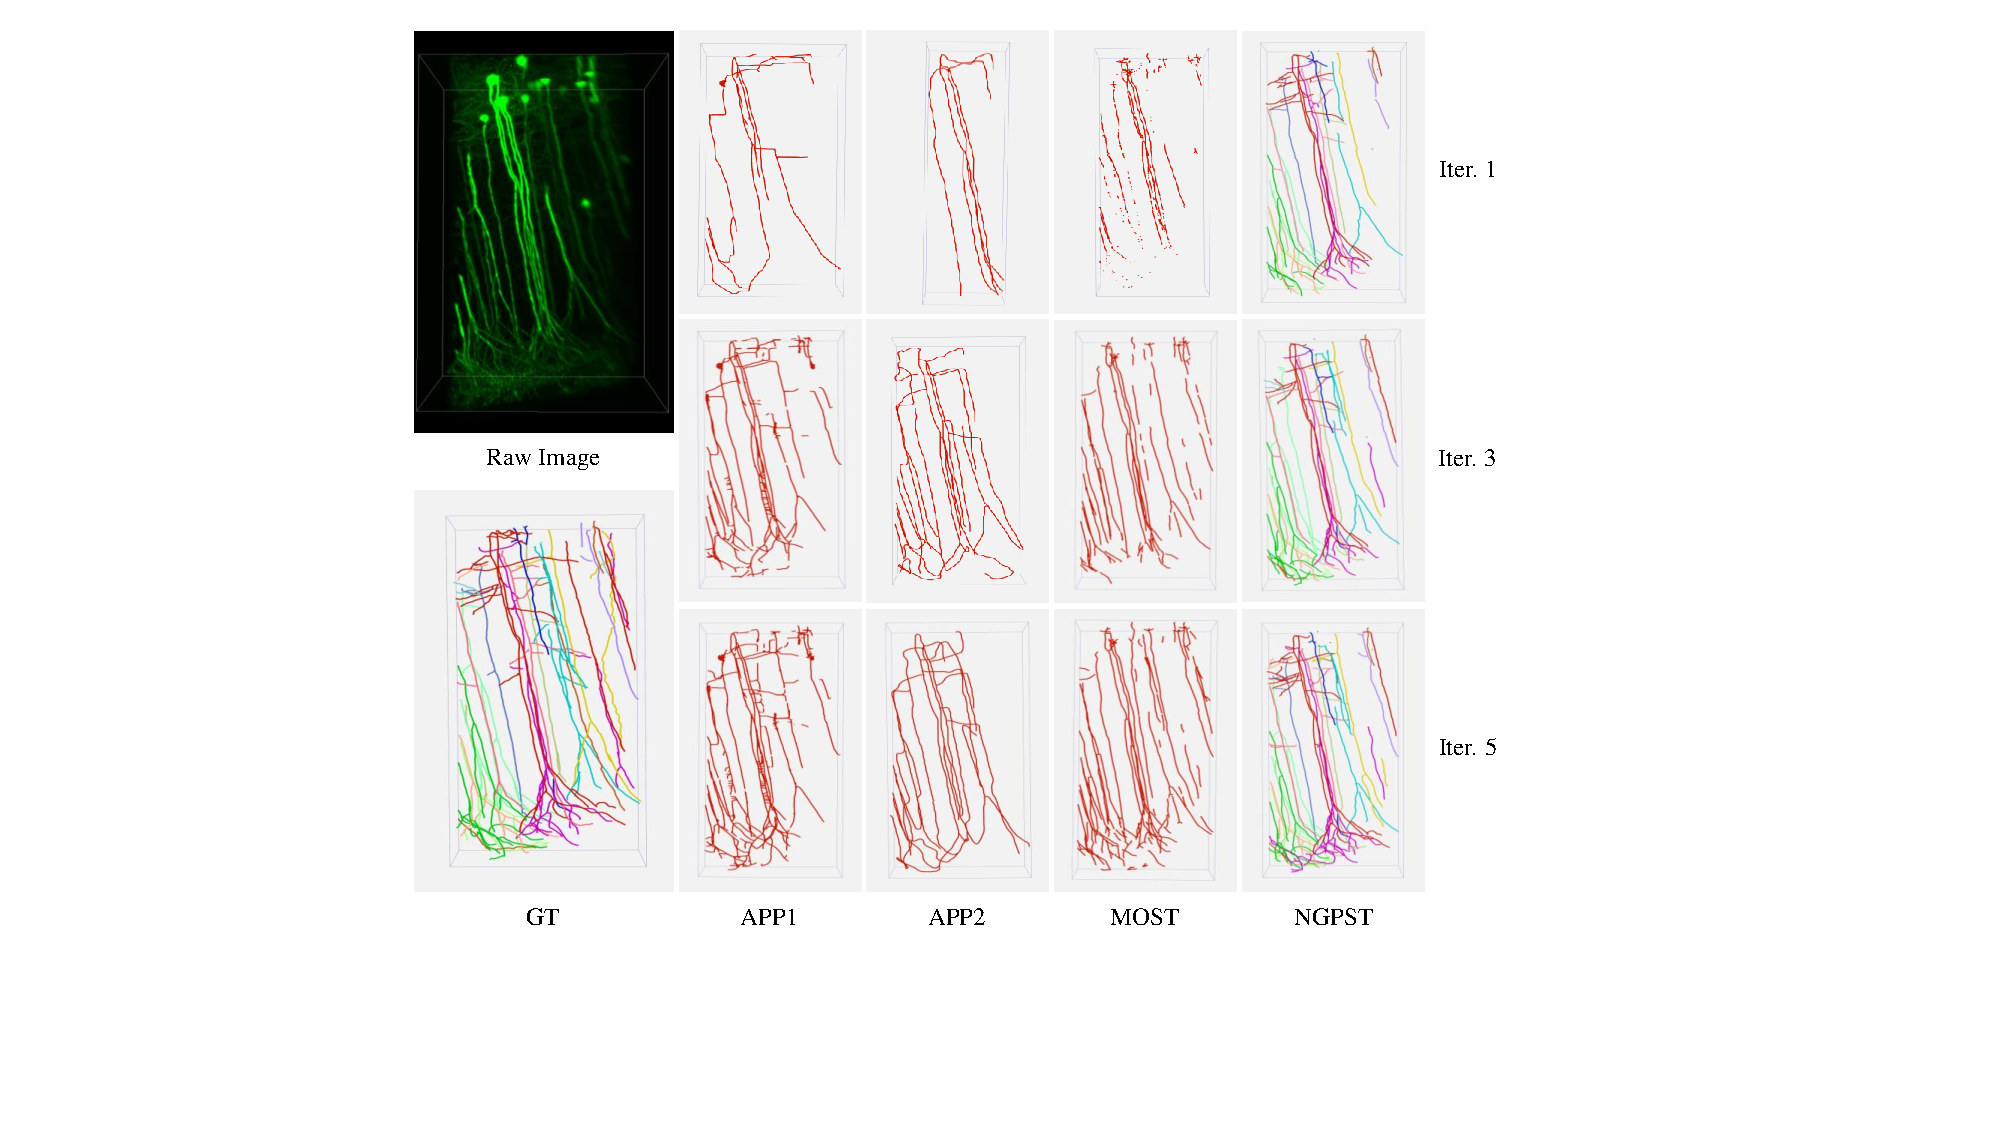
\includegraphics[width=1\columnwidth]{./Illustrations/trace_iterations3.pdf}
	\caption{Reconstruction results of the neuronal population in a test image from the VISoR-40 dataset at different iterations (top to bottom) using four neuron tracing methods APP1~\cite{Peng2011}, APP2~\cite{Xiao2013}, MOST\cite{Wu2014} and NGPST~\cite{Quan2015}.}
	\label{fig:trace_iterations}
\end{figure}

\begin{table}[t]
	\centering
	%\makeatletter\def\@captype{table}\makeatother
	\caption{F-Score of neuron reconstruction on a test image from the VISoR-40 dataset at different iterations using four neuron tracing methods APP1~\cite{Peng2011}, APP2~\cite{Xiao2013}, MOST\cite{Wu2014} and NGPST~\cite{Quan2015}.}
	\label{table:trace_iterations}
	\begin{tabular}{lccc}
		\toprule
		Method & iter-1 & iter-3 & iter-5\\
		\midrule
		APP1~\cite{Peng2011}
		& 0.315 & 0.599 & 0.599\\
		APP2~\cite{Xiao2013}
		& 0.251 & 0.511 & 0.538\\
		MOST~\cite{Wu2014}          
		& 0.322 & 0.588 & 0.721\\
		NGPST~\cite{Quan2015}
		& 0.758 & 0.825 & 0.888\\
		\bottomrule
	\end{tabular}
\end{table}

\begin{figure}[t]
	\centering
	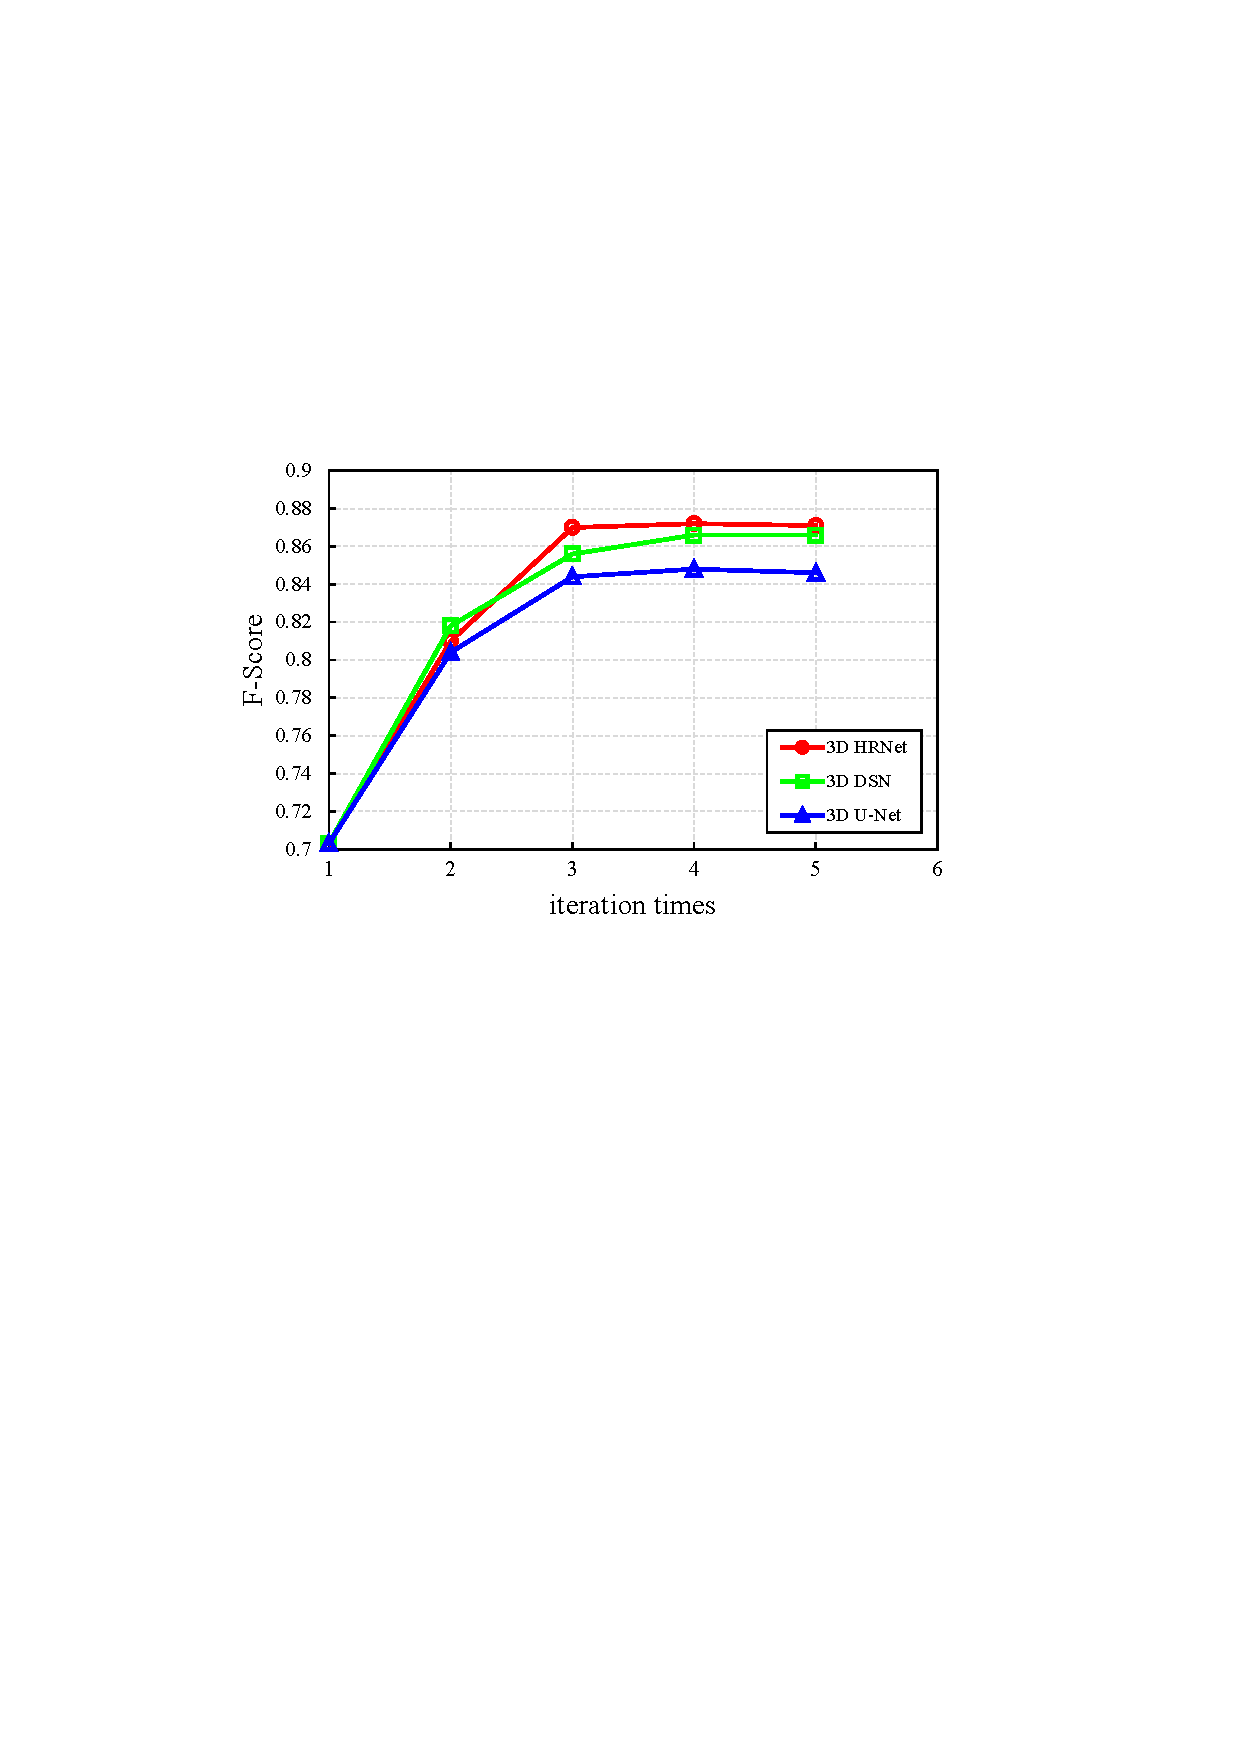
\includegraphics[width=\columnwidth]{./Illustrations/trace_networks_fscore11.pdf}
	\caption{F-Score of neuron reconstruction on the VISoR-40 test dataset at five iterations. Combining any one of the three neuron segmentation networks, our approach progressively improves the reconstruction performance.}
	\label{fig:fscore_DNNs}
\end{figure}

\begin{figure}[t]
	\centering
	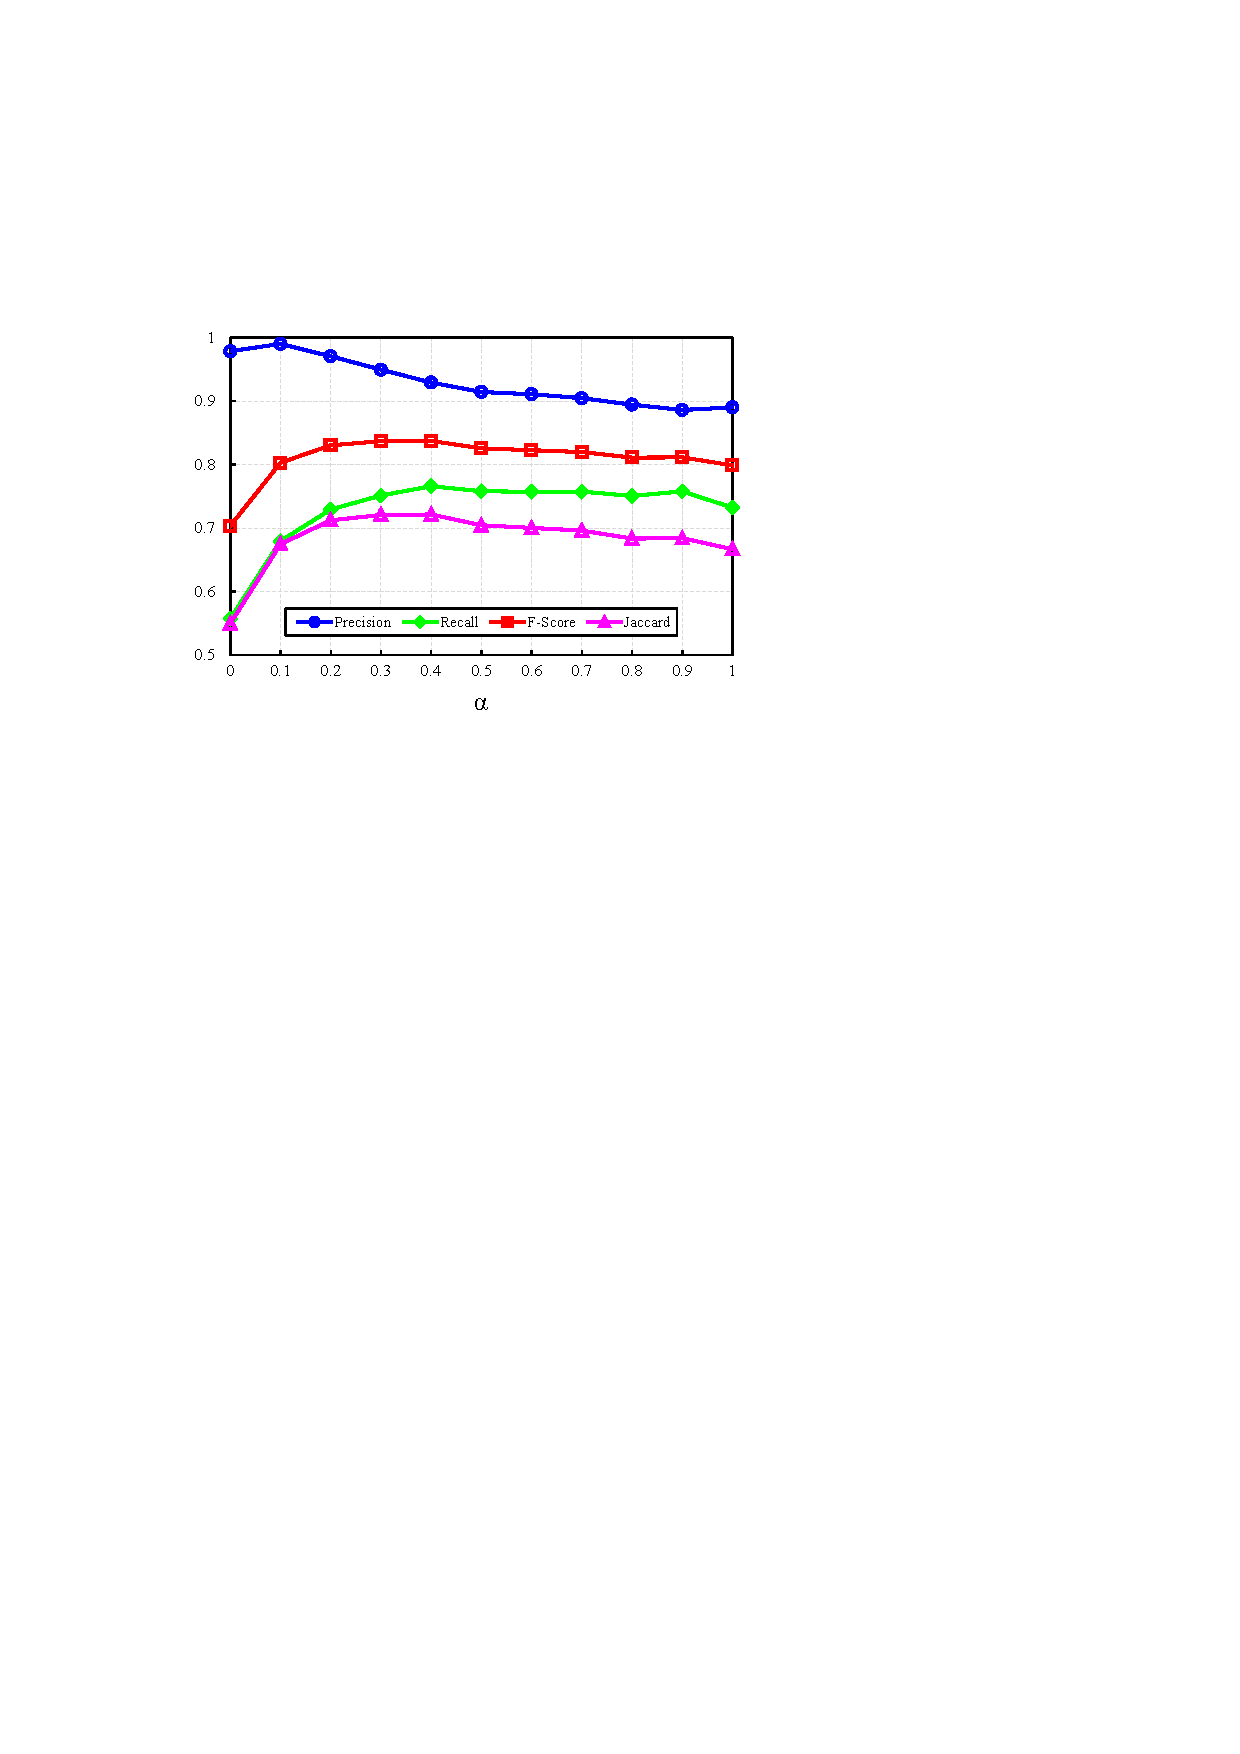
\includegraphics[width=\columnwidth]{./Illustrations/weight_paprameter7.pdf}
	\caption{Neuron reconstruction performance with different $\alpha$ in Eq.~\eqref{equ: enhance} for image enhancement on the VISoR-40 test dataset. From left to right, the value of $\alpha$ increases from $0$ to $1$ by a step of $0.1$.  }
	\label{fig:weight_paprameter}
\end{figure}

\begin{figure*}[t]
	\centering
	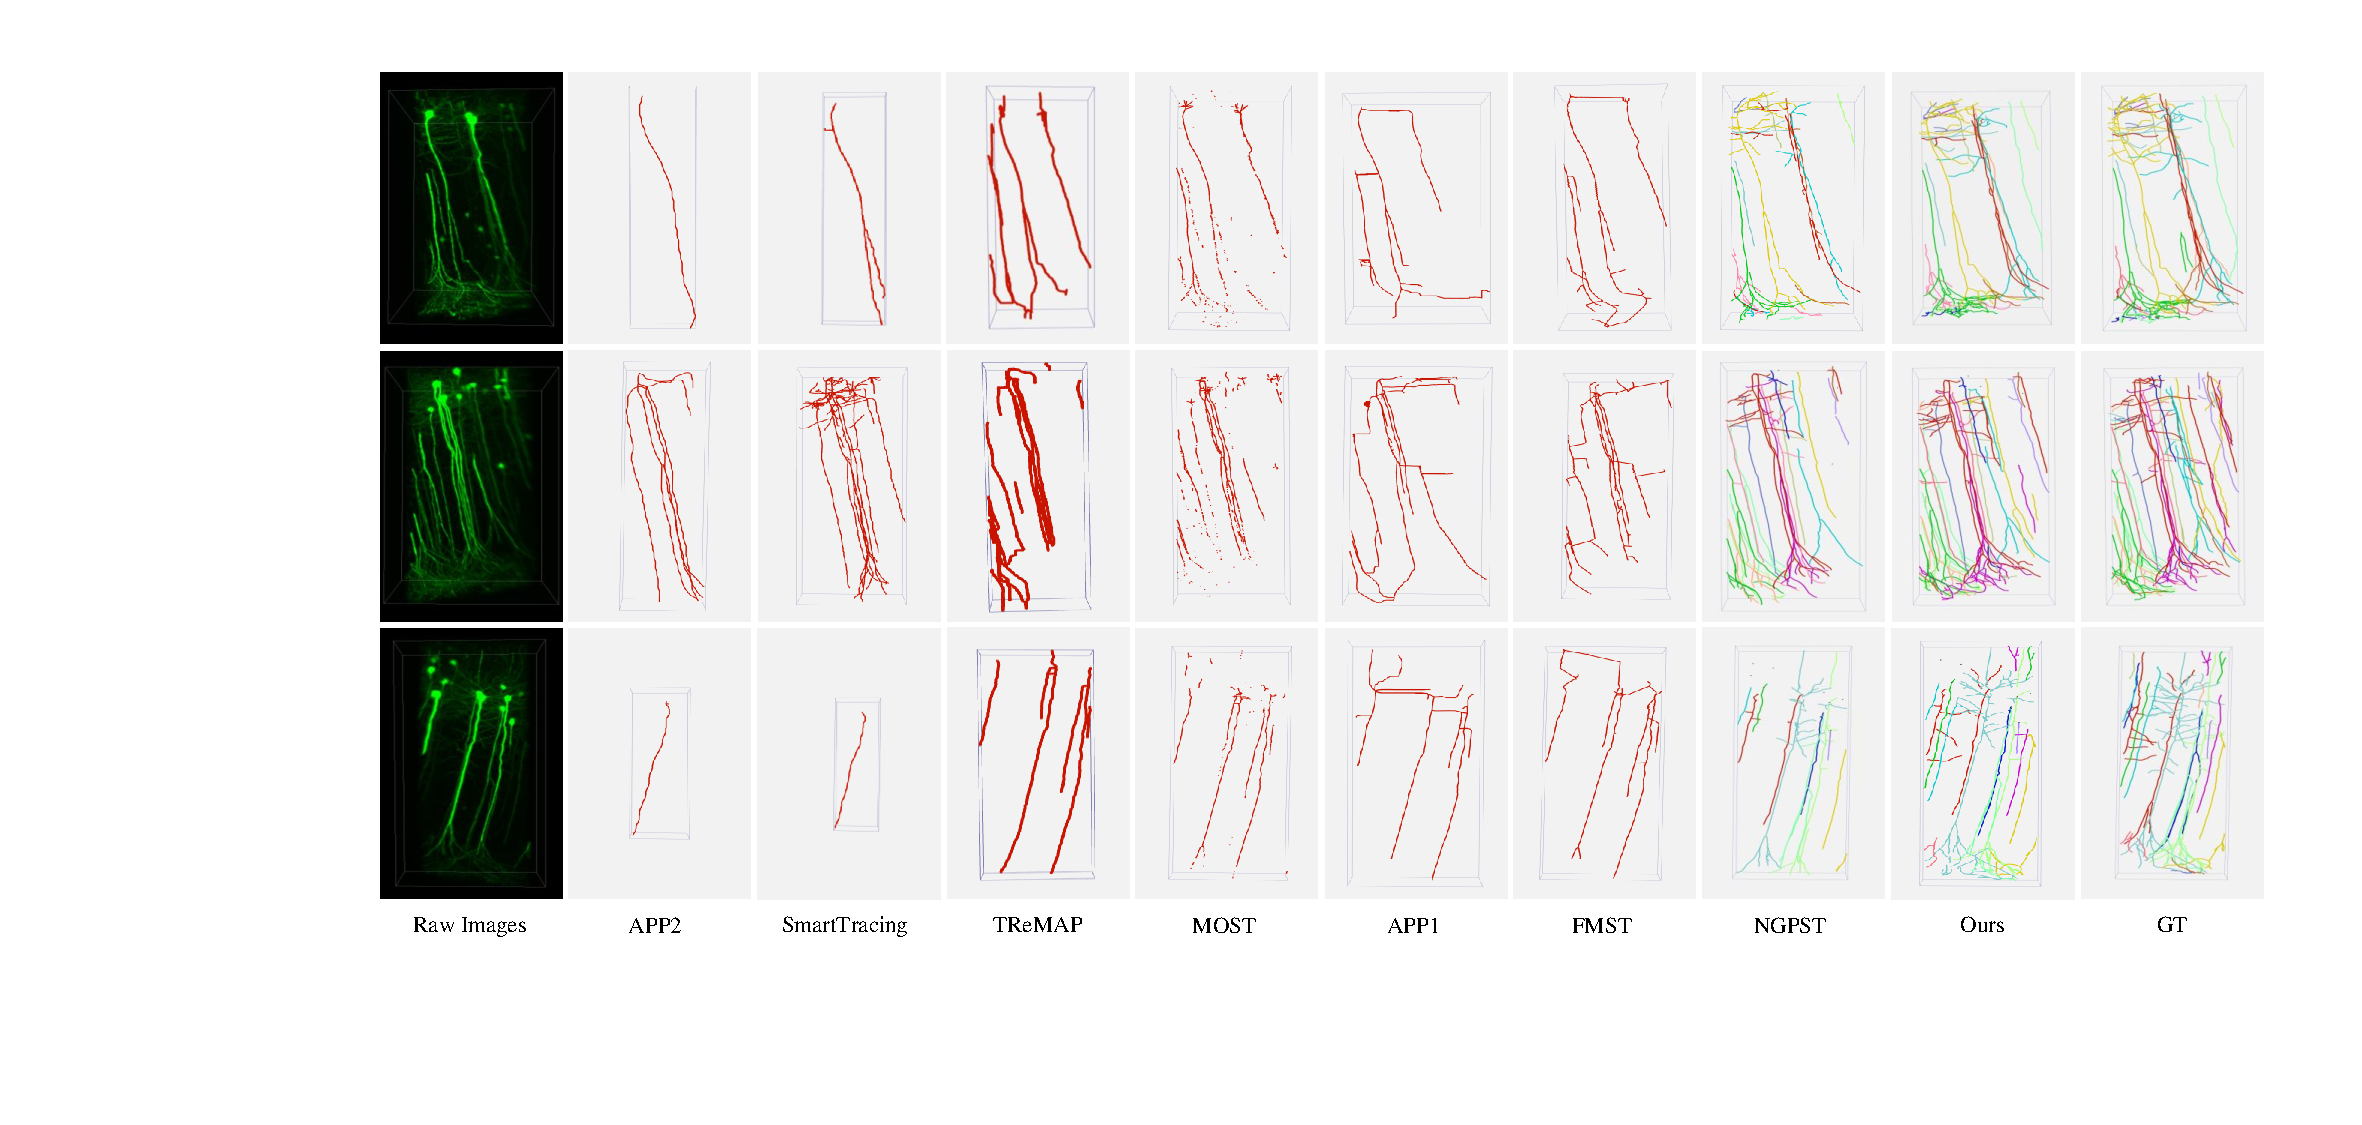
\includegraphics[width=1\textwidth]{./Illustrations/iteration3.pdf}
	\caption{Comparison of neuronal population reconstruction results using neuron reconstruction methods FMST~\cite{Yang2018}, APP1~\cite{Peng2011}, APP2~\cite{Xiao2013}, SmartTracing~\cite{Chen2015}, MOST~\cite{Wu2014}, NGPST~\cite{Quan2015} and our PLNPR on three test images from the VISoR-40 dataset.
	Each row shows the reconstruction results generated by different methods for a test image. The first column shows the raw images, while the last column shows the ground truth (GT). Each of the remaining columns shows the reconstruction result using the corresponding tracing method. We can observe that, our method reconstructs more complete and accurate neurons compared to other methods.
	%We can observe that, our method reconstructs more complete and accurate neuronal populations compared to other methods.
	}
	\label{fig:compare_VISoR}
\end{figure*}

\subsubsection{Progressive Learning}

The key idea of PLNPR is to progressively improve the performance of neuron reconstruction by making the neuron segmentation network and the conventional tracing method complementary and synergistic without using any manual annotations.
In order to demonstrate the performance improvement, four extensively used tracing methods are tested as the neuron tracing module in our framework. 
They are APP1~\cite{Peng2011}, APP2~\cite{Xiao2013}, MOST\cite{Wu2014} and NGPST~\cite{Quan2015} respectively. Their implementations are available in the software Vaa3D~\cite{Peng2014}. 
%
Eight iterations are tested on our VISoR-40 dataset, and the improvement of neuronal population reconstruction can be seen in the Fig.~\ref{fig:fscore_iterations}.
Here, we only show the F-Score which is widely used to reflect the overall performance of neuron reconstruction.
Moreover, the neuron reconstruction performance on a testing block at different iterations are shown in the Fig.~\ref{fig:trace_iterations} and \md{Table.~\ref{table:trace_iterations}}.
%
More qualitative and quantitative results are reported in the supplementary materials.
It can be observed that, our progressive learning strategy effectively facilitates conventional tracing methods to reconstruct more complete neuronal populations.
In addition, after about five iterations of the progressive learning, the reconstruction is relative complete and the room of performance improvement is becoming smaller with further iterations.

%\de{The key idea of PLNPR is to progressively learn features to extract neuron voxels from noisy backgrounds by utilizing a deep segmentation network with pseudo labels obtained by conventional tracing methods. This progressive learning strategy greatly improves neuronal population reconstruction performance without any annotations. We test four widely used techniques as the neuron tracing module in our framework. They are NGPST~\cite{Quan2015}, MOST\cite{Wu2014}, APP1~\cite{Peng2011} and its variant APP2~\cite{Xiao2013}, respectively. Their implementations are available in the software Vaa3D~\cite{Peng2014}. Each neuron tracing method is tested to produce pseudo labels for the training of the segmentation network on our VISoR-40 dataset. Eight iterations are tested, and the improvement of reconstruction performance using different neuron tracing methods is shown in Fig.~\ref{fig:fscore_iterations}.  Here, we only show the F-Score, which is commonly used to reflect the overall performance of the reconstruction results. Accordingly, Fig.~\ref{fig:trace_iterations} shows the reconstructed neurons on a test image at different iterations. More quantitative and qualitative results are reported in the supplementary materials. It can be seen that our progressive learning framework effectively facilitates conventional neuron tracing methods. Each tracing method is promoted to reconstruct more complete and accurate neurons.  In addition, after about five iterations of the progressive learning, the reconstruction is relatively complete, and further iteration just improves the performance very slightly.}



\subsubsection{Neuron Segmentation Network}

To further verify the effectiveness and robustness of our progressive learning strategy, we test three commonly used deep segmentation networks for extracting neuron voxels in our framework. They are 3D DSN~\cite{Dou2017}, 3D U-Net~\cite{Cicek2016} and a 3D version of HRNet~\cite{Sun2019}, respectively.
%All of them have the same input size, i.e. $160 \times 160\times 160$.
Five iterations are tested on our VISoR-40 dataset, and the F-Score of reconstruction results is shown in the Fig.~\ref{fig:fscore_DNNs}. 
%the improvement of reconstruction performance with different DNNs is shown in Fig.~\ref{fig:fscore_DNNs}.
It can be seen that our PLNPR algorithm can effectively improve the neuron reconstruction performance by combining any one of the three neuron segmentation networks.
The network and tracing method can complement and promote each other, leading to more complete reconstruction.


\subsubsection{Enhancement Parameter} 

In order to explore the influence of parameter $\alpha$ in Eq.~\eqref{equ: enhance} for image enhancement, we adopt different values for $\alpha$, and the results are shown in Fig.~\ref{fig:weight_paprameter}.
$\alpha=0$ means that the raw image block is directly used as input for the tracing module.
$\alpha=1$ means that only the probability maps are used as input for neuron tracing. 
It indicates that the performance is improved by combing the probability map with the raw intensity, mainly because that the probability map reflects the long-range trajectory structures while the original intensity preserves signal details to some extent.
%Second, it can be observed our system is very robust to the parameter $\alpha$. 
%Hence, the chosen of the parameter $\alpha$ is not very demanding and the reconstruction performance can achieve significant improvement with any $\alpha >0$. 
In this paper, we empirically select $\alpha=0.1$ to reduce the influence of false positive predictions in probability maps due to the limited performance of the DNN model trained by pseudo labels and increase the robustness of the whole framework.



\subsubsection{Comparison on VISoR-40 Dataset}

\begin{table*}[th]
	\centering
	\caption{Performance comparison with different methods for neuronal population reconstruction on the VISoR-40 dataset.}
	\label{table:compare_VISoR}
	\begin{tabular}{lcccc}
		\toprule
		Method & Precision & Recall & F-Score & Jaccard\\
		\midrule
		%\hline
		APP2~\cite{Xiao2013}
		& \textbf{0.980} & 0.091 & 0.157 & 0.091\\
		SmartTracing~\cite{Chen2015}
		& 0.961 & 0.133 & 0.205 & 0.128\\
		TReMAP~\cite{Zhou2016}
		& 0.917 & 0.147 & 0.253 & 0.145\\
		MOST~\cite{Wu2014}          
		& 0.969 & 0.151& 0.258& 0.151\\
		APP1~\cite{Peng2011}
		& 0.935 & 0.169 & 0.284 & 0.167\\
		FMST~\cite{Yang2018}
		& 0.884 & 0.179 & 0.296 &  0.176\\
		NGPST~\cite{Quan2015}
		& 0.978 & 0.557& 0.703 & 0.549\\
		\midrule
		Ours
		& 0.971 & \textbf{0.801}&\textbf{0.875} & \textbf{0.781}\\
		\bottomrule
	\end{tabular}
\end{table*}

%<18-AAAI-Adaptive Graph Convolutional Neural Networks>
To prove the effectiveness of our method on neuronal population reconstruction, we compare it with seven widely used neuron tracing methods, which include APP2~\cite{Xiao2013}, SmartTracing~\cite{Chen2015}, TReMAP~\cite{Zhou2016}, MOST~\cite{Wu2014}, APP1~\cite{Peng2011}, FMST~\cite{Yang2018} and NGPST~\cite{Quan2015}.
\md{The parameters of tracing methods are manually adjusted for each image to get optimal performance in the experiments.}
%
Table~\ref{table:compare_VISoR} compares the quantitative results of different methods with regard to Precision, Recall, F-Score and Jaccard.
``Ours'' means that we utilize NGPST with DSN enhancement after progressive learning on the VISoR-40 dataset.
From Table~\ref{table:compare_VISoR}, we can observe that our method makes a significant improvement compared with other methods.
%As can be seen from the table, our method makes a significant improvement compared with other methods.
%Fig.~\ref{fig:compare_VISoR} shows the neurons reconstructed from three testing images using different methods.
The neuronal populations reconstructed from three testing image blocks are visualized in Fig.~\ref{fig:compare_VISoR}.
It can be observed that our method outperforms others in both sparse and dense neurons.
Conventional methods~\cite{Xiao2013, Peng2011, Wu2014, Zhou2016} and machine learning based methods~\cite{Chen2015, Yang2018} tend to extract the main trunk of neurons, while missing a large portion of subtle neurites. 
Therefore, these methods have very high precision but significantly lower recall.
Although NGPST~\cite{Quan2015} has a better performance of neuronal identity, it still remains difficult to extract subtle neuron voxels by using hand-crafted features.
%
In comparison, our method benefits from the progressively trained DSN, and reconstructs more complete neurons from challenging blocks, even there exhibit noises, low contrast and blending of fluorescence in the blocks.
%\de{In order to validate the effectiveness of our PLNPR method on reconstructing dense neuronal population, we compare with seven widely used methods on our VISoR-40 dataset, including APP2~\cite{Xiao2013}, SmartTracing~\cite{Chen2015}, TReMAP~\cite{Zhou2016}, MOST~\cite{Wu2014}, APP1~\cite{Peng2011}, FMST~\cite{Yang2018} and NGPST~\cite{Quan2015}. Table~\ref{table:compare_VISoR} shows the quantitative results of our method, compared with the seven methods. ``Ours" means that we use NGPST with DSN enhancement after progressive learning on the VISoR-40 dataset. It can be observed that our method makes a significant improvement compared with the second best result~\cite{Quan2015}. Fig.~\ref{fig:compare_VISoR} shows the reconstructed neurons using different methods on three test images. It can be seen that our method outperforms others in both sparse and dense neurons. APP1~\cite{Peng2011}, APP2~\cite{Xiao2013}, SmartTracing~\cite{Chen2015} and MOST~\cite{Wu2014} tend to extract the main trunk of the neurons while a large portion of subtle neurites are missing. Therefore, these methods lead to very high precision but significantly lower recall. NGPST works better to identity dense neurons. However, subtle neurites are still hard to extract by using hand-crafted features. In comparison, our method benefits from the progressively trained DSN, and reconstructs more complete and accurate neurons from challenging images, even there exhibit low contrast, noises, and blending of fluorescence in the images.}




\subsection{Evaluation of PLNPR on BigNeuron Dataset}
\label{sec:exp_PLNPR_BigNeuron}

\subsubsection{BigNeuron Dataset}

To validate our PLNPR method on the single neuron reconstruction, we employ the BigNeuron~\cite{peng2015} dataset which is a well-known community-derived neuron dataset. 
This dataset totally consists of about $ 20,000 $ 3D OM images, acquired from a variety of species and optical imaging systems.
Some images have the corresponding manual annotations for evaluation.
Unlike our VISoR-40 dataset which is built for the evaluation of neuronal population reconstruction, each block in the BigNeuron dataset contains a single neuron or fragmented neurites which is appropriate for single neuron reconstruction.
\md{In this work, 68 images we used from the BigNeuron dataset are the same as Li2017~\cite{Li2017}. These images are from a variety of species, and each image has the corresponding expert manual reconstruction. $ 3/4 $ of these images are sampled for network training and the remaining images are used for evaluation to compute the neuron tracing performance.}


\subsubsection{Experimental Settings and Evaluation Metrics}
 
\md{
We evaluate the proposed progressive learning method on the single neuron reconstruction application. The DSN model is progressively trained on the VISoR-40 dataset first and then fine-tuned on the BigNeuron dataset using pseudo labels generated by NGPST~\cite{Quan2015} instead of the provided manual annotations.
The learning rate was initialized as $\num{1e-4} $ and decayed using the ``poly" learning rate policy. The maximum iteration number is set to $ 24000 $.
We cropped patches of size $160\times 160\times 8$ as input to the network, considering consumption of the GPU memory, and also unequal image sizes along three directions.
}

\md{
Since the implementation of most learning-based tracing methods, such as~\cite{Li2017} are not publicly available, to compare with~\cite{Li2017}, the testing data and three evaluation metrics for evaluation are the same as those used in~\cite{Li2017}.
The three measurements defined in~\cite{Peng2010a} include entire structure average (ESA), different structure average (DSA) and percentage of different structures (PDS). For all of these three scores, larger values indicate higher discrepancy between the tracing results and the manual reconstruction.
}
%Specifically, they are calculated in following ways. For each node in manual reconstruction, we 从 calculated the minimal spatial distance between this node and all nodes in the reconstructed nodes generated by computational methods. The ESA is obtained by averaging all these reciprocal minimal spatial distances; the DSA only sums those distances that are larger than 2 voxels since the difference of two nodes that is less than 2 voxels is hardly distinguished visually. The PDS captures the percentage of pairs of nodes whose reciprocal minimal spatial distances are more than 2 voxels.


\subsubsection{Comparison on BigNeuron Dataset}

\begin{figure*}[th]
	\centering
	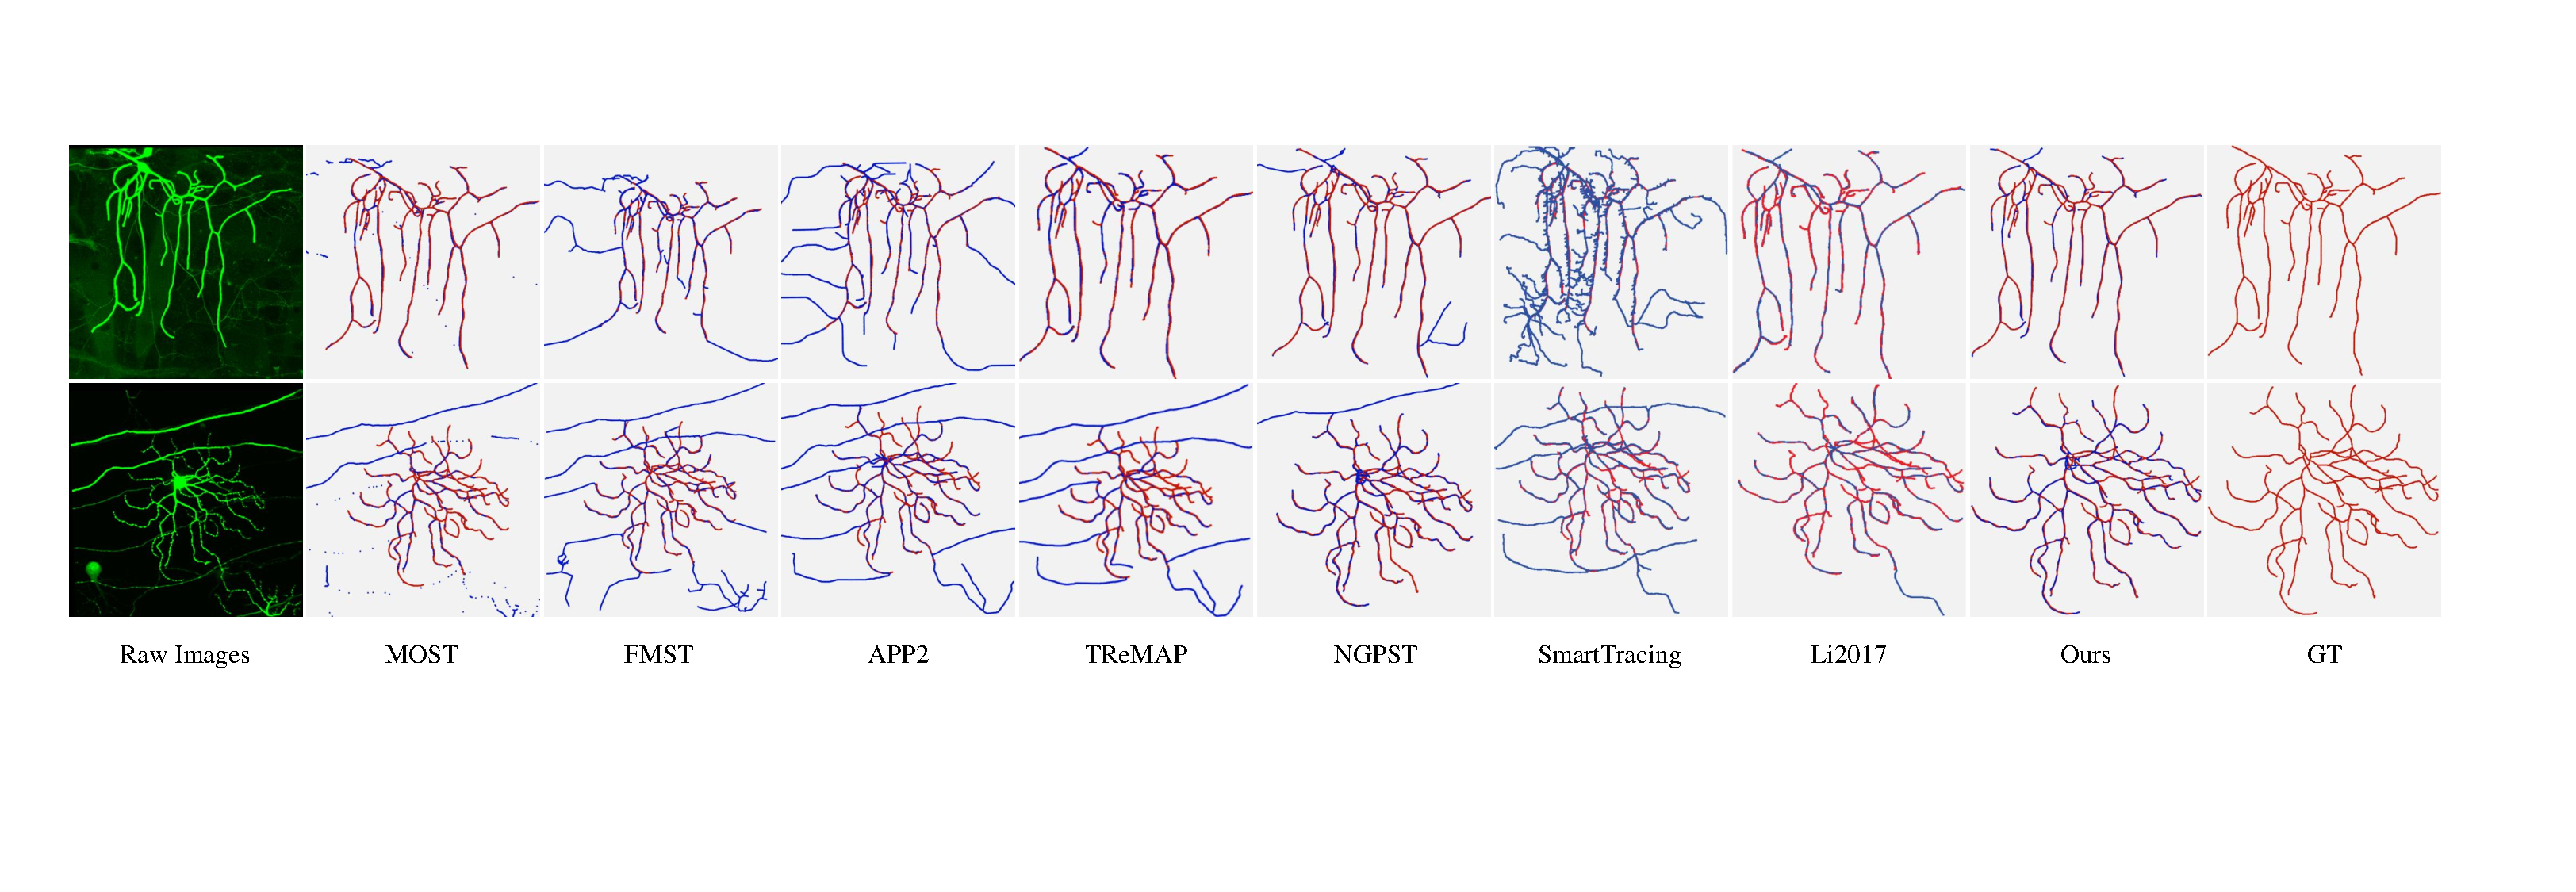
\includegraphics[width=1\textwidth]{./Illustrations/BigNeuron6.pdf}
	\caption{Comparison of single neuron reconstruction results using MOST~\cite{Wu2014}, FMST~\cite{Yang2018}, APP2~\cite{Xiao2013}, TReMAP~\cite{Zhou2016}, NGPST~\cite{Quan2015}, SmartTracing~\cite{Chen2015}, Li2017~\cite{Li2017} and our PLNPR on two testing images from the BigNeuron dataset.
	%Each row shows the reconstruction results generated by different methods for a test image. The first column shows the raw images, while the last column shows the ground truth (GT). Each of the remaining columns shows the reconstruction result using the corresponding tracing method. 
	Here, we overlay each reconstruction result in blue with the corresponding ground truth (GT) which are denoted by red.
	We can observe that, our method reconstructs more complete and accurate neurons compared to other methods.
	}
	\label{fig:compare_BigNeuron}
\end{figure*}

\delete{
\begin{table*}[t]
	\centering
	\makeatletter\def\@captype{table}\makeatother\caption{Performance comparison %in terms of entire structure %average (ESA), different structure average (DSA) and percentage of different structures (PDS) 
		with different methods for single neuron reconstruction on the BigNeuron dataset.}\label{table:compare_BigNeuron2}
	\begin{tabular}{lcccccc}  
		\toprule
		\multirow{2}*{Method}  & \multicolumn{3}{c}{test image 1} & \multicolumn{3}{c}{test image 2} \\ 
		\cline{2-7}
		& ESA & DSA & PDS & ESA & DSA & PDS\\
		\midrule
		MOST~\cite{Wu2014} & 31.730 & 38.211 & 0.633 & 31.730 & 38.211 & 0.633\\
		\midrule
		Ours & \textbf{4.784} & 8.309 & \textbf{0.451} & \textbf{4.784} & 8.309 & \textbf{0.451}\\
		\bottomrule
	\end{tabular}
\end{table*}

FMST~\cite{Yang2018} & 17.878 & 23.459 & 0.558\\
	APP2~\cite{Xiao2013} & 13.457 & 17.923 & 0.562\\
	TReMAP~\cite{Zhou2016} & 11.269 & 17.941 & 0.539\\
	NGPST~\cite{Quan2015} & 10.168 & 14.880 & 0.587\\
	SmartTracing~\cite{Chen2015} & 8.532 & 11.609 & 0.543\\
	Li2017~\cite{Li2017} & 4.917 & \textbf{7.972} &0.461 \\
}

\begin{table*}[th]
	\centering
	\makeatletter\def\@captype{table}\makeatother
	\caption{Performance comparison in terms of Precision, Recall, F-Score, Jaccard, entire structure average (ESA), different structure average (DSA) and percentage of different structures (PDS) with different methods for single neuron reconstruction on the BigNeuron test dataset.}
	\label{table:compare_BigNeuron}
	\begin{tabular}{lccccccc}
		\toprule
		Method & Precision & Recall & F-Score & Jaccard & ESA & DSA & PDS\\
		\midrule
		MOST~\cite{Wu2014} & 0.619 & 0.361 & 0.456 & 0.295 & 31.730 & 38.211 & 0.633\\
		FMST~\cite{Yang2018} & 0.575 & 0.629 & 0.601 & 0.429 & 17.878 & 23.459 & 0.558\\
		APP2~\cite{Xiao2013} & \textbf{0.799} & 0.492 & 0.608 & 0.437 & 13.457 & 17.923 & 0.562\\
		TReMAP~\cite{Zhou2016} & 0.771 & 0.415 & 0.539 & 0.369 & 11.269 & 17.941 & 0.539\\
		NGPST~\cite{Quan2015} & 0.710 & 0.680 & 0.695 & 0.532 & 10.168 & 14.880 & 0.587\\
		SmartTracing~\cite{Chen2015} & 0.701 & 0.648 & 0.674 & 0.508 & 8.532 & 11.609 & 0.543\\
		Li2017~\cite{Li2017} & - & - & - & - & 4.917 & \textbf{7.972} &0.461 \\
		\midrule
		Ours & 0.790 & \textbf{0.707} & \textbf{0.746}  & \textbf{0.595} & \textbf{4.784} & 8.309 & \textbf{0.451}\\
		\bottomrule
	\end{tabular}
\end{table*}

\begin{figure}[t]
	\centering
	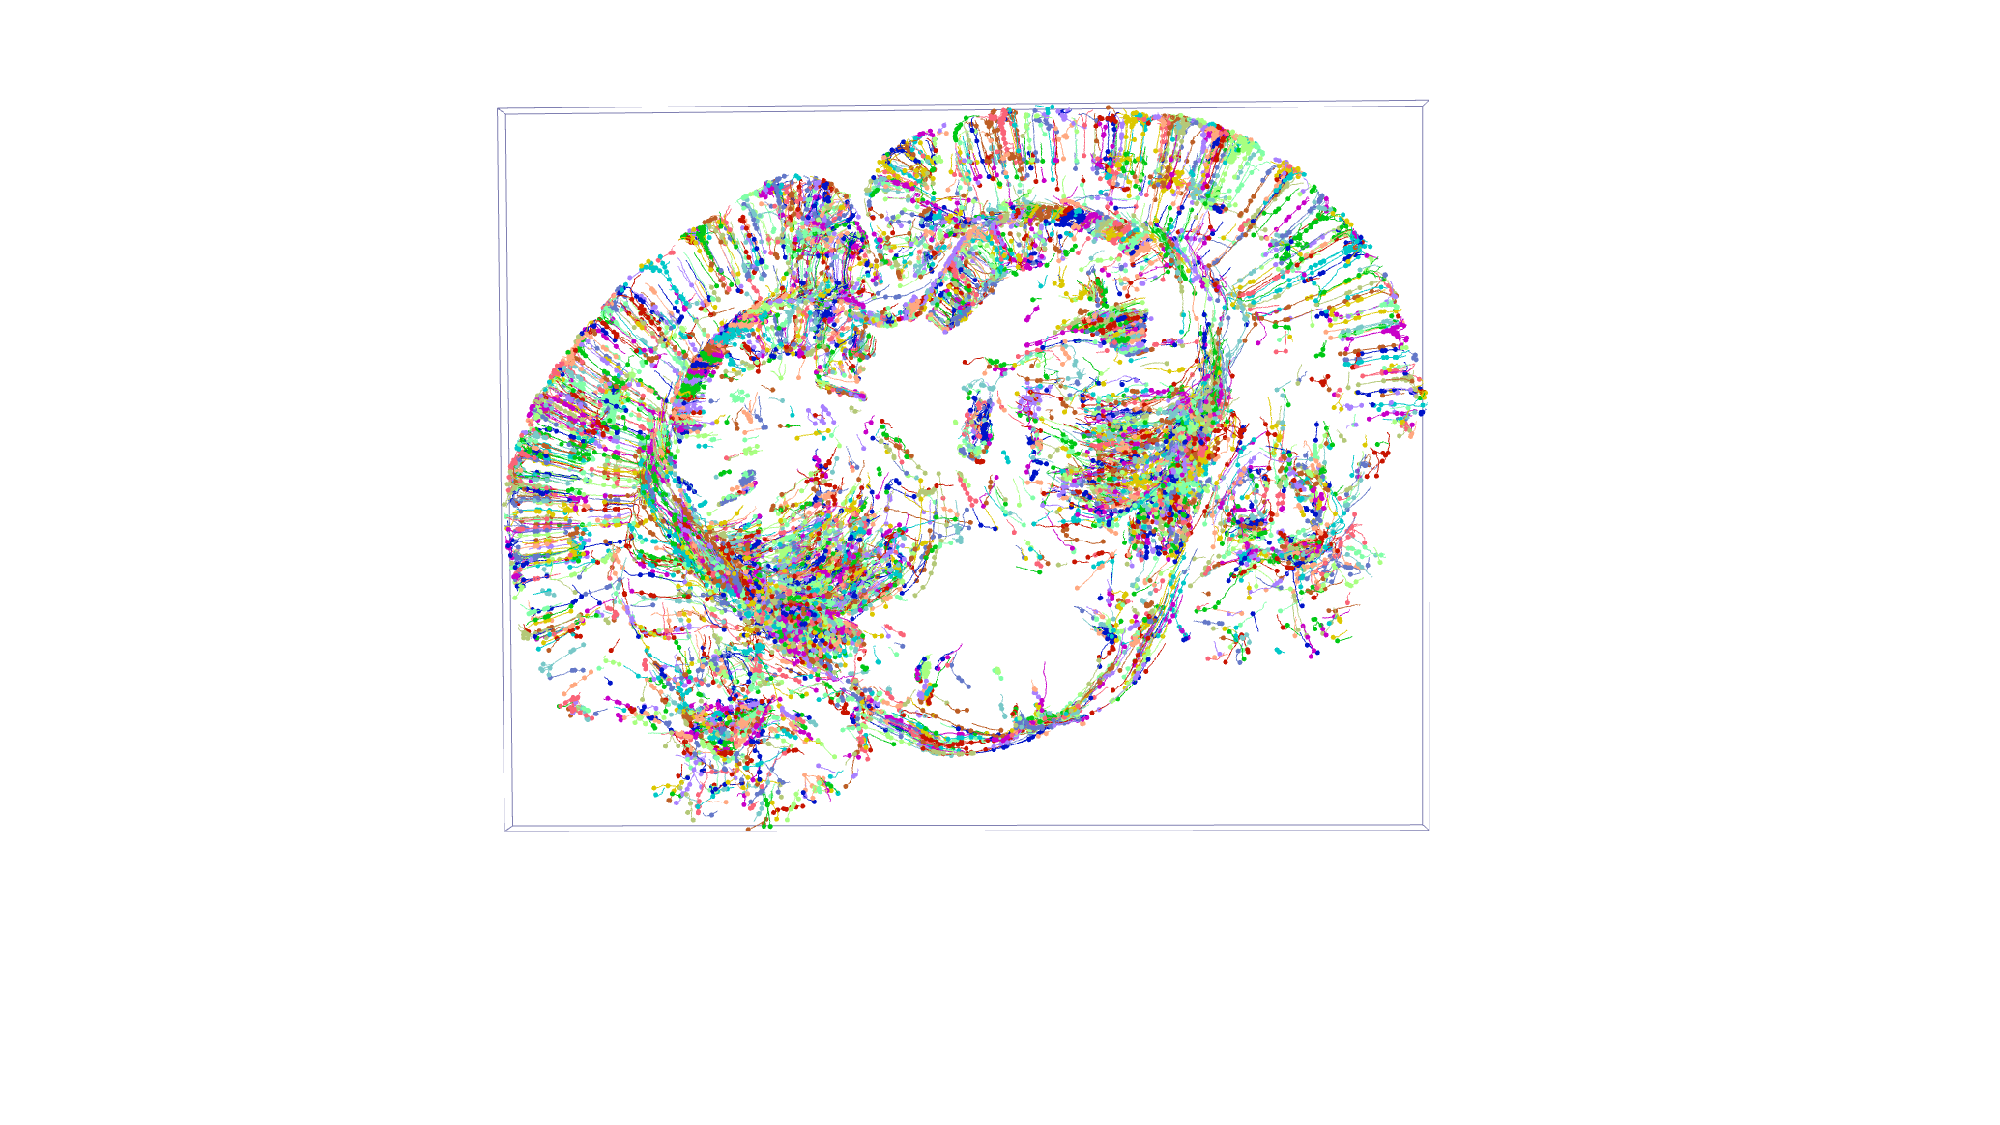
\includegraphics[width=1\columnwidth]{./Illustrations/brain_slice.pdf}
	\caption{The reconstruction result of neuronal populations in a large-scale 3D mouse brain slice using our UltraNPR method.}
	\label{fig:reconstruct_brain}
\end{figure}


On the BigNeuron dataset, we compare with seven widely used tracing methods to validate the effectiveness of our proposed method.
They are MOST~\cite{Wu2014}, FMST~\cite{Yang2018}, APP2~\cite{Xiao2013}, TReMAP~\cite{Zhou2016}, NGPST~\cite{Quan2015}, SmartTracing~\cite{Chen2015} and Li2017~\cite{Li2017}, respectively.
%To compare with the deep learning based method, the testing data and three evaluation metrics for evaluation are the same as those used in~\cite{Li2017}. The three measurements include different structure average (DSA), percentage of different structures (PDS) and entire structure average (ESA).
Fig.~\ref{fig:compare_BigNeuron} visualizes the neurons reconstructed from two testing blocks.
%``Ours'' means that we utilize NGPST with DSN, which is progressively trained on the VISoR-40 dataset first and then fine-tuned on the BigNeuron dataset using pseudo labels instead of the provided manual annotations.
%It can be seen that
Our method reconstructs more accurate neuronal morphology compared with other methods.
%The weighted average of the ESA, DSA and PDS on all testing images are listed in Table~\ref{table:compare_BigNeuron}.
In Table~\ref{table:compare_BigNeuron}, we list the weighted average of the DSA, PDS and ESA on all testing data using different methods.
%The weights are proportional to the neuron lengths identified in manual annotations.
The weight of each testing block is proportional to the neuron length identified in the corresponding manual annotation.
From Table~\ref{table:compare_BigNeuron}, we can observe that our method outperforms others in both PDS and ESA metrics and also achieves comparable performance in DSA metric with the best one.
In particular, unlike~\cite{Li2017} requiring on a strongly supervised network, our method obtains even better performance without any manual annotations.
With ever-increasing number of unlabeled neuron datasets are collected, our method can easily utilize them to further improve the performance of neuron reconstruction.

%\delete{To further validate the effectiveness of our PLNPR method, we also compare our results with seven methods on the BigNeuron~\cite{peng2015} dataset, including MOST~\cite{Wu2014}, FMST~\cite{Yang2018}, APP2~\cite{Xiao2013}, TReMAP~\cite{Zhou2016}, NGPST~\cite{Quan2015}, SmartTracing~\cite{Chen2015} and Li2017~\cite{Li2017}. For a fair comparison with deep learning based method, we use the testing data and three evaluation metrics the same as~\cite{Li2017}. Specifically, these metrics are entire structure average (ESA), different structure average (DSA) and percentage of different structures (PDS). Fig.~\ref{fig:compare_BigNeuron} shows the reconstruction results using different methods on two test images. The weighted average of the ESA, DSA and PDS on all test images of different methods are reported in Table~\ref{table:compare_BigNeuron}. The weights are proportional to the neuron lengths identified in the ground truth. ``Ours" means that we use NGPST with DSN enhancement after progressive learning on the VISoR-40 dataset first and then finetuned on BigNeuron dataset using pseudo labels rather than using the provided annotations. It can be seen that our method outperforms others in both ESA and PDS metrics and also achieves comparable performance in DSA metric with the best one. In particular, different from the supervised deep learning based method~\cite{Li2017}, our PLNPR gets even better performance without using any manual annotations. With ever increasing amounts of unlabeled microscopic datasets are collected, our method can easily utilize these datasets to further improve the performance of neuron reconstruction.}

\subsection{Evaluation of UltraNPR on a Mouse Brain Slice}
\label{sec:exp_UltraNPR}

%\subsubsection{Experimental Settings}
We use our UltraNPR algorithm to reconstruct a neuronal population from a large-scale OM brain image. 
The image used in this work is shown in Fig.~\ref{fig:brain}, a mouse brain slice with image resolution of $25397\times 18516\times 869$ ($761$GB), in which a large number of neurons are densely distributed. Considering the image size and the computational efficiency, the block size is set to be $1120\times 2048\times 869$.  The overlap between adjacent blocks is set to be $300$ voxels.
%In addition, we introduce $300$ voxels overlap between adjacent blocks to avoid false continuation and increase the robustness of the reconstruction.
%
%In this work, the This image from a mouse brain slice contains $25397\times 18516\times 869$ voxels ($761$GB in size), in which a large number of neurons are densely distributed, as shown in Fig.~\ref{fig:brain}.
%Fig.~\ref{fig:brain} shows an MIP along axial dimension of the brain slice. This OM image was captured by the VISoR imaging system~\cite{Wang2019}, with a image resolution of $25397\times 18516\times 869$ and a physical resolution of $0.5 \times0.5 \times 0.5$ \SI{}{\micro\metre}$^3$ per voxel, which makes it capable to visualize individual neurons. 
UltraNPR is performed on the full image and takes just over one day to reconstruct the image on a cluster computer with $64$ GB of working memory and 20 NVIDIA 1080Ti GPUs.
As shown in Fig.~\ref{fig:reconstruct_brain}, a neuronal population is successfully reconstructed from the large-scale image, which consists of $5348$ neurons.
%There are $5348$ neurons been reconstructed and $4886$ somas been detected.
%\md{The quality of the tracking results depends on brian region that is selected from the image. We found that UltraNPR works better in the regions that have }
\begin{figure}[t]
	\centering
	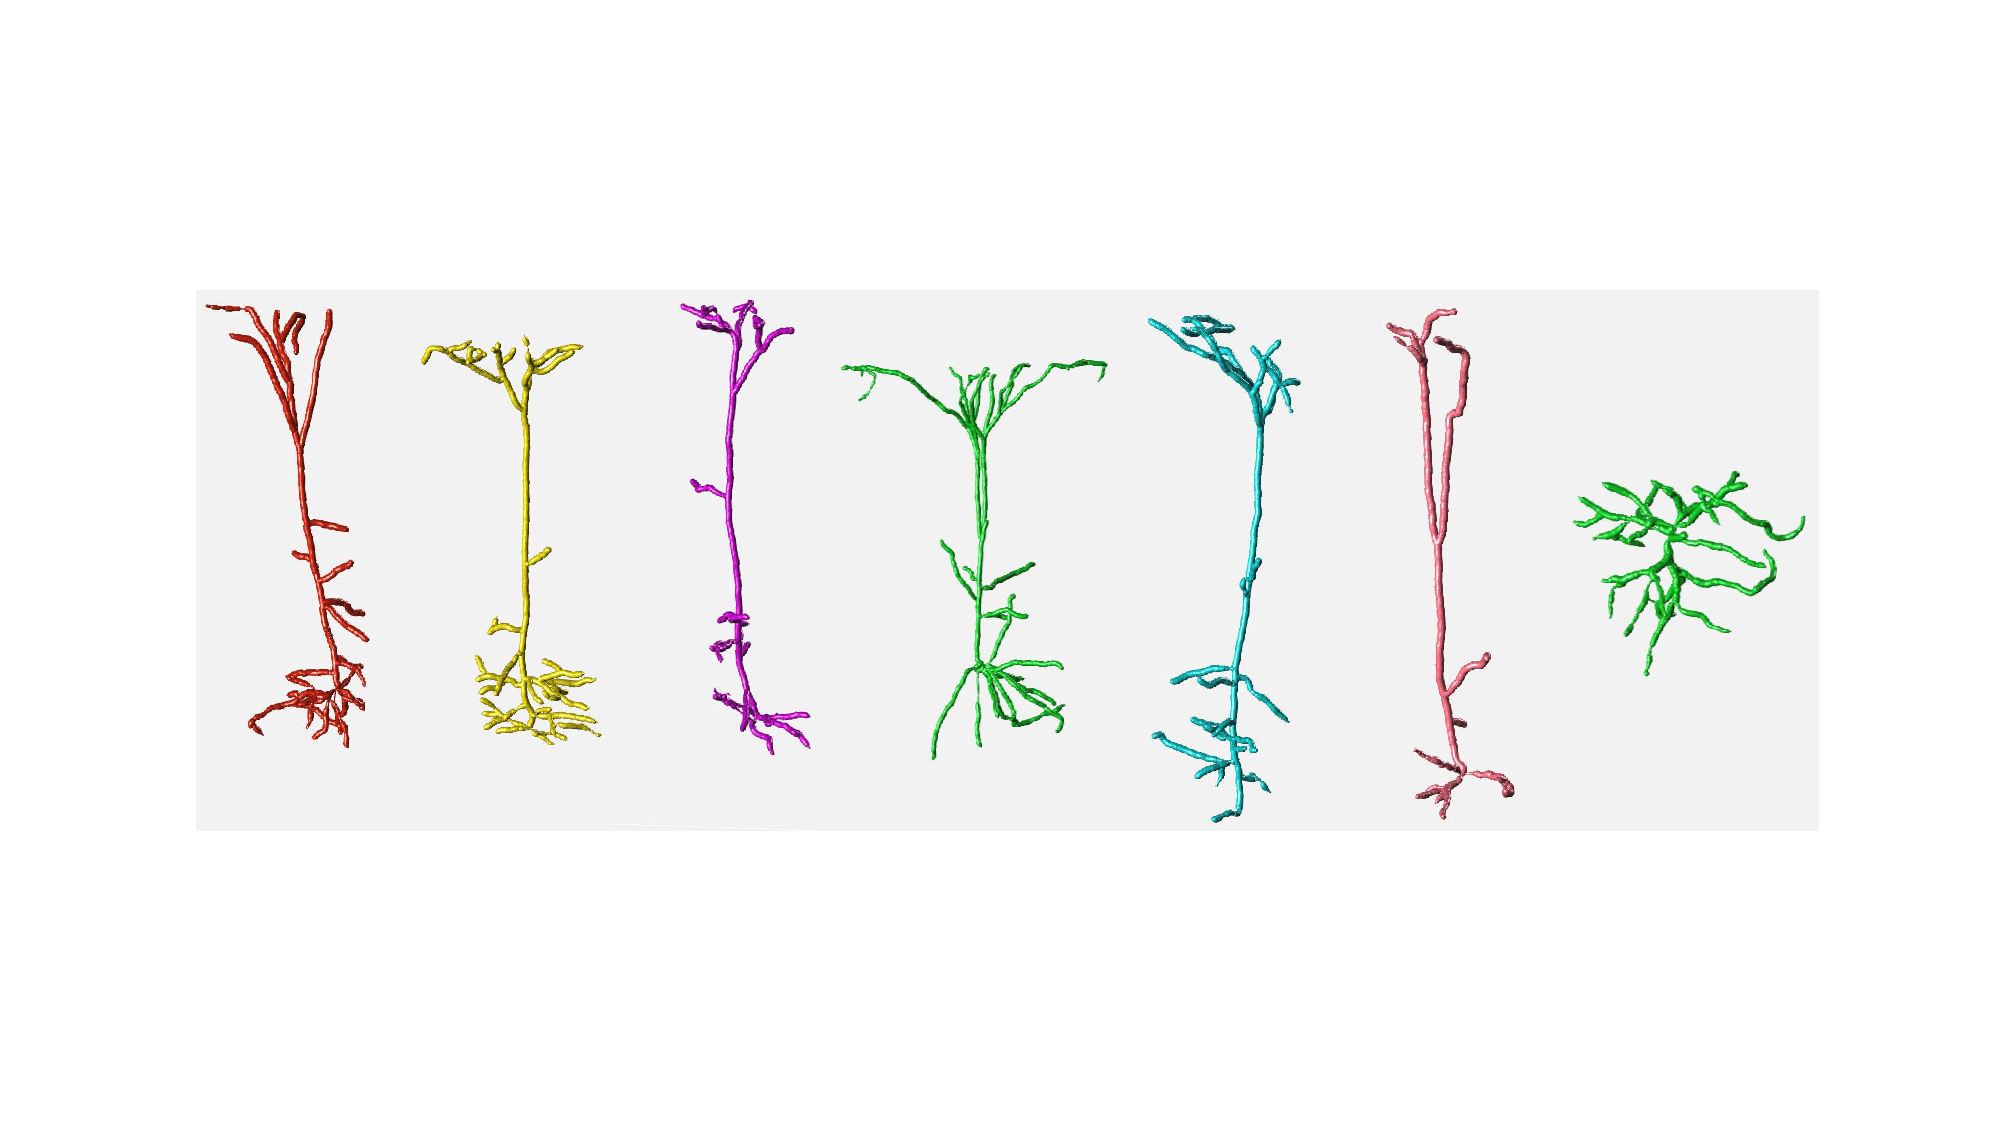
\includegraphics[width=1\columnwidth]{./Illustrations/single_neurons4.pdf}
	\caption{Single neurons selected from the reconstructed neuronal populations in a mouse brain slice using our UltraNPR method.}
	\label{fig:single_neurons}
\end{figure}

\md{brain region}
Several neurons selected from the reconstructed neuronal population are visualized in Fig.~\ref{fig:single_neurons}. These reconstructions provide detailed neuronal structures and enable further neuronal morphology analysis. 
In summery, our results suggest that UltraNPR is capable of reconstructing neuronal populations from noisy and large-scale OM brain images.

Neuron length, number of branches.

\md{Since the manual annotation of neuronal populations from noisy OM images is difficult to obtain, let along the annotation of large-scale neuronal populations from a mouse brain slice. In this section, some qualitative results are visualized for verifying the effectiveness of our UltraNPR method.}